
\pdfminorversion=4

~% if handout is on %~
    \documentclass[professionalfonts,handout]{beamer}
    \setbeameroption{show notes}
    \setbeamertemplate{note page}{\insertnote}
    \setbeamercolor{background canvas}{bg=white}
~% else %~
    ~% if interactive is on %~
        \documentclass[professionalfonts,handout]{beamer}
    ~% else %~
        \documentclass[professionalfonts]{beamer}
    ~% endif %~
~% endif %~



% Template original the Beamer: Copyright 2004 by Till Tantau <tantau@users.sourceforge.net>.


\mode<presentation>
{
  \usetheme{metropolis}
  % or ...

  %\setbeamercovered{transparent} %hace que lo que esta covered se muestre transparente
}

\setbeamertemplate{navigation symbols}{}%remove navigation symbols

\usepackage[english]{babel}

\usepackage[latin1]{inputenc}

\usepackage{times}
\usepackage[T1]{fontenc}

% para poder escribir codigo fuente en las diapositivas
\usepackage{listings}

% para graficar diagramas simples y arboles de jerarquias
\usepackage{tikz}
\usepackage{tikz-qtree}
\usetikzlibrary{matrix,positioning}
\usetikzlibrary{shapes,arrows,chains,calc,decorations.pathmorphing,decorations.shapes}

\definecolor{myLightGray}{RGB}{191,191,191}
\definecolor{myGray}{RGB}{160,160,160}
\definecolor{myDarkGray}{RGB}{144,144,144}
\definecolor{myDarkRed}{RGB}{167,114,115}
\definecolor{myRed}{RGB}{255,58,70}
\definecolor{myGreen}{RGB}{0,255,71}

\usepackage{xcolor}
\definecolor{darkgreen}{rgb}{0,.5,0}
\definecolor{darkblue}{rgb}{0,0,.7}
\lstdefinestyle{normal}{language=C++,       % lenguaje C++
   numbers=left,                            % enumerar las lineas
   keywordstyle=\color{darkblue}\textbf,    % color de las keywords
   stringstyle=\color{red},                 % color de los strings
   commentstyle=\color{darkgreen},          % color de los comentarios
   basicstyle=\color{black}\ttfamily\footnotesize\bfseries,     % color del texto en general
   morecomment=[l][\color{magenta}]{\#},    % coloreamos las intrucciones del precompilador (todo lo que empieza con #)
   ndkeywords={NULL,nullptr,siz,zer,mov,add,noexcept},               % definimos una nuevas keywords como NULL y nullptr
   ndkeywordstyle=\color{violet},           % y las nuevas keywords tendran este color
   frame=simple,                            % simple, sin ningun marco o frame alrededor del codigo
   basewidth={0.55em,0.55em}                % tamano de las letras/lineas. usado para reducir el whitespace entre estas
}

\lstdefinestyle{normal33}{language=C++,       % lenguaje C++
   numbers=left,                            % enumerar las lineas
   keywordstyle=\color{darkblue}\textbf,    % color de las keywords
   stringstyle=\color{red},                 % color de los strings
   commentstyle=\color{darkgreen},          % color de los comentarios
   basicstyle=\color{black}\ttfamily\footnotesize\bfseries,     % color del texto en general
   morecomment=[l][\color{magenta}]{\#},    % coloreamos las intrucciones del precompilador (todo lo que empieza con #)
   ndkeywords={NULL,nullptr},               % definimos una nuevas keywords como NULL y nullptr
   ndkeywordstyle=\color{violet},           % y las nuevas keywords tendran este color
   frame=simple,                            % simple, sin ningun marco o frame alrededor del codigo
   basewidth={0.55em,0.55em}                % tamano de las letras/lineas. usado para reducir el whitespace entre estas
}
%mismo estilo, sin numeros
\lstdefinestyle{normalnonumbers}{language=C++,
   keywordstyle=\color{darkblue}\textbf,
   stringstyle=\color{red},
   commentstyle=\color{darkgreen},
   basicstyle=\color{black}\ttfamily\footnotesize\bfseries,
   morecomment=[l][\color{magenta}]{\#},
   ndkeywords={NULL,nullptr,move,add},
   ndkeywordstyle=\color{violet},
   frame=simple,
   basewidth={0.55em,0.55em}
}


% mismo estilo pero todos los colores estan mas debiles como si se volvieran transparentes
% usado para poder resaltar el codigo.
\lstdefinestyle{dimmided}{language=C++,
   keywordstyle=\color{darkblue!30}\textbf,
   stringstyle=\color{red!30},
   commentstyle=\color{darkgreen!30},
   basicstyle=\color{black!30}\ttfamily\footnotesize\bfseries,
   morecomment=[l][\color{magenta!30}]{\#},
   ndkeywords={NULL,nullptr,siz,zer,mov,add},
   ndkeywordstyle=\color{violet!30},
   moredelim=**[is][\only<+->{\color{black}\lstset{style=normal}}]{@}{@}, % definimos que las lineas entre arrobas (@) tendran el estilo normal (con los colores a toda intensidad)
   frame=simple,
   basewidth={0.55em,0.55em}
}
\lstdefinestyle{dimmided42}{language=C++,
   keywordstyle=\color{darkblue!30}\textbf,
   stringstyle=\color{red!30},
   commentstyle=\color{darkgreen!30},
   basicstyle=\color{black!30}\ttfamily\footnotesize\bfseries,
   morecomment=[l][\color{magenta!30}]{\#},
   ndkeywords={NULL,nullptr,siz,zer,mov,add},
   ndkeywordstyle=\color{violet!30},
   moredelim=**[is][{\color{black}\lstset{style=normal}}]{@}{@}, % definimos que las lineas entre arrobas (@) tendran el estilo normal (con los colores a toda intensidad)
   frame=simple,
   basewidth={0.55em,0.55em}
}

\lstdefinelanguage{json}{
    literate=
     *{:}{{{\color{violet}{:}}}}{1}
      {,}{{{\color{violet}{,}}}}{1}
      {\{}{{{\color{darkgreen}{\{}}}}{1}
      {\}}{{{\color{darkgreen}{\}}}}}{1}
      {[}{{{\color{darkgreen}{[}}}}{1}
      {]}{{{\color{darkgreen}{]}}}}{1},
}


\lstdefinestyle{normaljson}{language=json,  % lenguaje json
   numbers=left,                            % enumerar las lineas
   keywordstyle=\color{darkblue}\textbf,    % color de las keywords
   stringstyle=\color{red},                 % color de los strings
   commentstyle=\color{red},                % color de los comentarios
   basicstyle=\color{black}\ttfamily\footnotesize\bfseries,     % color del texto en general
   morecomment=[l][\color{magenta}]{\#},    % coloreamos las intrucciones del precompilador (todo lo que empieza con #)
   ndkeywords={NULL,nullptr},               % definimos una nuevas keywords como NULL y nullptr
   ndkeywordstyle=\color{violet},           % y las nuevas keywords tendran este color
   frame=simple,                            % simple, sin ningun marco o frame alrededor del codigo
   basewidth={0.55em,0.55em}                % tamano de las letras/lineas. usado para reducir el whitespace entre estas
}

\lstdefinelanguage{http}{
    morekeywords={
        GET,
        PUT,
        POST,
        DELETE
    }
}

\lstdefinestyle{normalhttp}{language=http,  % lenguaje HTTP
   numbers=left,                            % enumerar las lineas
   keywordstyle=\color{darkblue}\textbf,    % color de las keywords
   stringstyle=\color{red},                 % color de los strings
   commentstyle=\color{red},                % color de los comentarios
   basicstyle=\color{black}\ttfamily\footnotesize\bfseries,     % color del texto en general
   morecomment=[l][\color{magenta}]{\#},    % coloreamos las intrucciones del precompilador (todo lo que empieza con #)
   ndkeywords={NULL,nullptr},               % definimos una nuevas keywords como NULL y nullptr
   ndkeywordstyle=\color{violet},           % y las nuevas keywords tendran este color
   frame=simple,                            % simple, sin ningun marco o frame alrededor del codigo
   basewidth={0.55em,0.55em}                % tamano de las letras/lineas. usado para reducir el whitespace entre estas
}

% Pone las constantes numericas con color (violeta en este caso):
% - los numeros que estan dentro de un string/comentarios NO son coloreados
% - los numeros por fuera que pertenecen a una palabra SON coloreados
%   (buf1, por ejemplo, el "1" es coloreado cuando no lo deberias. UPS!!)
% - No incluye el signo
%
%\lstset{literate=%
%  *{0}{{{\color{violet}0}}}1
%   {1}{{{\color{violet}1}}}1
%   {2}{{{\color{violet}2}}}1
%   {3}{{{\color{violet}3}}}1
%   {4}{{{\color{violet}4}}}1
%   {5}{{{\color{violet}5}}}1
%   {6}{{{\color{violet}6}}}1
%   {7}{{{\color{violet}7}}}1
%   {8}{{{\color{violet}8}}}1
%   {9}{{{\color{violet}9}}}1
%}

% Para resaltar lineas de codigo usando \btLstHLB{range} y \btLstHLB<overlay>{range}:
% Por ejemplo,
%  \btLstHLB{3}       linea 3 resaltada
%  \btLstHLB{1-5}     lineas de la 1 a la 5 resaltadas
%  \btLstHLB<2>{3}    linea 3 resaltada solo en el slide 2
%
% \btLstHLB usa un color azul mientras que \btLstHLR usa un color rojo como fondo
\usepackage{lstlinebgrd}
\makeatletter
\newcount\bt@rangea
\newcount\bt@rangeb

\newcommand\btIfInRange[2]{%
   \global\let\bt@inrange\@secondoftwo%
   \edef\bt@rangelist{#2}%
   \foreach \range in \bt@rangelist {%
      \afterassignment\bt@getrangeb%
      \bt@rangea=0\range\relax%
      \pgfmathtruncatemacro\result{ ( #1 >= \bt@rangea) && (#1 <= \bt@rangeb) }%
      \ifnum\result=1\relax%
      \breakforeach%
      \global\let\bt@inrange\@firstoftwo%
      \fi%
   }%
   \bt@inrange%
}
\newcommand\bt@getrangeb{%
   \@ifnextchar\relax%
   {\bt@rangeb=\bt@rangea}%
   {\@getrangeb}%
}
\def\@getrangeb-#1\relax{%
   \ifx\relax#1\relax%
      \bt@rangeb=100000%   \maxdimen is too large for pgfmath
   \else%
      \bt@rangeb=#1\relax%
   \fi%
}

%%%%%%%%%%%%%%%%%%%%%%%%%%%%%%%%%%%%%%%%%%%%%%%%%%%%%%%%%%%%%%%%%%%%%%%%%%%%%%
%
% \btLstHL<overlay spec>{range list}
%
\newcommand<>{\btLstHLB}[1]{%
   \only#2{\btIfInRange{\value{lstnumber}}{#1}{\color{blue!30}}% blue
   {\def\lst@linebgrdcmd####1####2####3{}}}%
}%
\newcommand<>{\btLstHLR}[1]{%
   \only#2{\btIfInRange{\value{lstnumber}}{#1}{\color{red!30}}% red
   {\def\lst@linebgrdcmd####1####2####3{}}}%
}%
%
%
%%%%%%%%%%%%%%%%%%%%%%

\makeatother


% sin fecha
\date{}

\author[7542-9508]{Di Paola Mart\'in \\ \texttt{martinp.dipaola <at> gmail.com} }

\institute[Universidad de Buenos Aires]
{
   Facultad de Ingenier\'ia\\
   Universidad de Buenos Aires
}

% Definimos una imagen para que este en cada slide
%\pgfdeclareimage[height=0.5cm]{university-logo}{imgs/fiuba.png}
%\logo{\pgfuseimage{university-logo}}

%% Definir estas en el documento final
%%
%% \title%
%% {Programaci\'on gen\'erica y templates en C++}
%%
%% \subject{Programaci\'on gen\'erica y templates en C++}


%%%%%
~% if interactive is on %~
    \AtBeginSection{}
    \AtBeginSubsection{}
~% else %~
    % At begin of each Section do nothing; at each Subsection show the Section and Subsection names
    % If the Section doesn't have a Subsection, then YOU must to add a unnumbered Subsection like \subsection*{}
    % so the AtBeginSubsection will get triggered
    \AtBeginSection{}
    \AtBeginSubsection[\frame{\subsectionpage}]{\frame{\subsectionpage}}
~% endif %~
%
%%%%%




\title%
{Memoria en C/C++}

\subject{Memoria en C/C++}

\begin{document}

\begin{frame}
   \titlepage
\end{frame}

\begin{frame}{De qu\'e va esto?}
   \tableofcontents
   % You might wish to add the option [pausesections]
\end{frame}

\section{Memoria}
\subsection{Tama\~nos, Alineaci\'on y Padding}
% sizeof int, char, char*, alineacion y padding
\begin{frame}[fragile,label=RM]{Exacta reserva de memoria}
   \begin{columns}
      \begin{column}{.55\linewidth}
         \begin{lstlisting}[style=dimmided]
@char c = 'A';@@
int i = 1;@@
short int s = 4;@@
char *p = 0;
int *g = 0;@@
int b[2] = {1, 2};@@
char a[] = "AB";@
         \end{lstlisting}
   \begin{itemize}
      \item<1-> Todo depende de la arquitectura y del compilador
      \item<2-> Alineaci\'on y padding
      \item<4-> Punteros del mismo tama\~no
      \item<6-> Un cero como "fin de string"
   \end{itemize}

      \end{column}
      \begin{column}{.05\linewidth}
      \end{column}
      \begin{column}{.30\linewidth}
         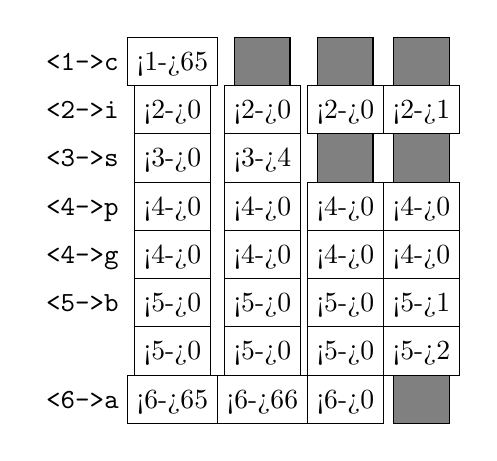
\begin{tikzpicture}[cell/.style={rectangle,draw=black},
            space/.style={minimum height=1.5em,matrix of nodes,row sep=-\pgflinewidth,column sep=-\pgflinewidth,column 1/.style={font=\ttfamily}},text depth=0.5ex,text height=2ex,nodes in empty cells]

            \matrix (first)[space, column 1/.style={font=\ttfamily},column 2/.style={nodes={cell,minimum width=2em}},column 3/.style={nodes={cell,minimum width=2em}},column 4/.style={nodes={cell,minimum width=2em}},column 5/.style={nodes={cell,minimum width=2em}}]
            {
               {\visible<1->{c}}   & {\visible<1->{65}} & |[fill=gray]| &  |[fill=gray]| &  |[fill=gray]| \\
               {\visible<2->{i}}   & {\visible<2->{0}} & {\visible<2->{0}} & {\visible<2->{0}} & {\visible<2->{1}}\\
               {\visible<3->{s}}   & {\visible<3->{0}} & {\visible<3->{4}} & |[fill=gray]|  & |[fill=gray]| \\
               {\visible<4->{p}}   & {\visible<4->{0}} & {\visible<4->{0}} & {\visible<4->{0}} & {\visible<4->{0}}\\
               {\visible<4->{g}}   & {\visible<4->{0}} & {\visible<4->{0}} & {\visible<4->{0}} & {\visible<4->{0}}\\
               {\visible<5->{b}}   & {\visible<5->{0}} & {\visible<5->{0}} & {\visible<5->{0}} & {\visible<5->{1}}\\
                                   & {\visible<5->{0}} & {\visible<5->{0}} & {\visible<5->{0}} & {\visible<5->{2}}\\
               {\visible<6->{a}}   & {\visible<6->{65}} & {\visible<6->{66}} & {\visible<6->{0}} & |[fill=gray]|\\
            };
         \end{tikzpicture}
      \end{column}
   \end{columns}
\end{frame}
\note[itemize] {
\item C y C++ son lenguajes de bajo nivel para que el programador pueda tener un control absoluto de d\'onde y c\'omo se ejecuta el c\'odigo.
\item El tama\~no en bytes de los tipos depende de la arquitectura y del compilador
\item El compilador puede guardar las variables en posiciones de memoria m\'ultiplos de 4 (depende de la arquitectura y de los flags de compilaci\'on): variables alineadas son accedidas m\'as r\'apidamente que las desalineadas.
\item Como contra, la alineaci\'on despedicia espacio (padding) hay un tradeoff entre velocidad y espacio.
\item El tama\~no de un puntero no depende de a que tipo apunta; todos los punteros ocupan el mismo tama\~no (que depende de la arquitectura).
\item A los strings en C escritos en el c\'odigo del programa el compilador les agrega el caracter nulo (byte 0). Tenerlo en cuenta!!
}


\begin{frame}[fragile]{Agrupaci\'on de variables}
   \begin{columns}
      \begin{column}{.55\linewidth}
         \begin{lstlisting}[style=normal]
struct S {
   int  a;
   char b;
   int  c;
   char d;
};

struct S s = {1,2,3,4};

         \end{lstlisting}
      \end{column}
      \begin{column}{.40\linewidth}
         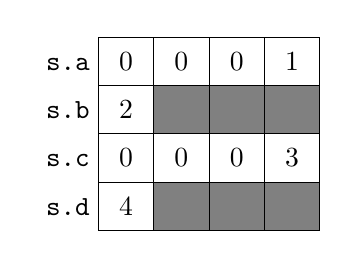
\begin{tikzpicture}[cell/.style={rectangle,draw=black},
            space/.style={minimum height=1.5em,matrix of nodes,row sep=-\pgflinewidth,column sep=-\pgflinewidth,column 1/.style={font=\ttfamily}},text depth=0.5ex,text height=2ex,nodes in empty cells]

            \matrix (first)[space, column 1/.style={font=\ttfamily},column 2/.style={nodes={cell,minimum width=2em}},column 3/.style={nodes={cell,minimum width=2em}},column 4/.style={nodes={cell,minimum width=2em}},column 5/.style={nodes={cell,minimum width=2em}}]
            {
               {s.a}   & {0} & {0} & {0} & {1}\\
               {s.b}   & {2} & |[fill=gray]| &  |[fill=gray]| &  |[fill=gray]| \\
               {s.c}   & {0} & {0} & {0} & {3}\\
               {s.d}   & {4} & |[fill=gray]| &  |[fill=gray]| &  |[fill=gray]| \\
            };
         \end{tikzpicture}
      \end{column}
   \end{columns}
\end{frame}
\note[itemize] {
\item El padding se hace mas notorio en las estructuras: el acceso a cada atributo es r\'apido pero hay memoria desperdiciada.
}

\begin{frame}[fragile]{Agrupaci\'on de variables}
   \begin{columns}
      \begin{column}{.55\linewidth}
         \begin{lstlisting}[style=normal]
struct S {
   int  a;
   char b;
   int  c;
   char d;
} __attribute__((packed));

struct S s = {1,2,3,4};

         \end{lstlisting}
      \end{column}
      \begin{column}{.45\linewidth}
         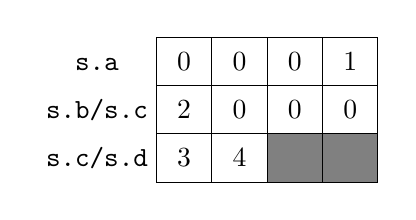
\begin{tikzpicture}[cell/.style={rectangle,draw=black},
            space/.style={minimum height=1.5em,matrix of nodes,row sep=-\pgflinewidth,column sep=-\pgflinewidth,column 1/.style={font=\ttfamily}},text depth=0.5ex,text height=2ex,nodes in empty cells]

            \matrix (first)[space, column 1/.style={font=\ttfamily},column 2/.style={nodes={cell,minimum width=2em}},column 3/.style={nodes={cell,minimum width=2em}},column 4/.style={nodes={cell,minimum width=2em}},column 5/.style={nodes={cell,minimum width=2em}}]
            {
               {s.a}       & {0} & {0} & {0} & {1}\\
               {s.b/s.c}   & {2} & {0} & {0} & {0}\\
               {s.c/s.d}   & {3} & {4} & |[fill=gray]| & |[fill=gray]|\\
            };
         \end{tikzpicture}
      \end{column}
   \end{columns}
\end{frame}
\note[itemize] {
\item Con el atributo especial de gcc \lstinline[style=normal]!__attribute__((packed))! el compilador empaqueta los campos sin padding, m\'as eficiente en memoria pero m\'as lento.
\item Y es m\'as lento por que para leer el atributo \lstinline[style=normal]!s.c! hay que hacer 2 lecturas.
\item Y cuidado, en algunas arquitecturas la lectura de atributos desalineados hace crashear al programa!
}

% endianess
\begin{frame}[fragile]{Endianess: representaci\'on en memoria}
   \begin{columns}
      \begin{column}{.05\linewidth}
         \begin{lstlisting}[style=normal]
int i = 1;





int j = 1023;
         \end{lstlisting}
      \end{column}
      \begin{column}{.05\linewidth}
      \end{column}
      \begin{column}{.3\linewidth}
         \vspace*{0.5mm}
         \begin{lstlisting}[style=normalnonumbers]
((unsigned char*)&i)
   == {0, 0, 0, 1}

((unsigned char*)&i)
   == {1, 0, 0, 0}
         \end{lstlisting}
         \vspace*{5mm}
         \begin{lstlisting}[style=normalnonumbers]
((unsigned char*)&j)
   == {0, 0, 3, 255}

((unsigned char*)&j)
   == {255, 3, 0, 0}
         \end{lstlisting}
      \end{column}
      \begin{column}{.4\linewidth}
         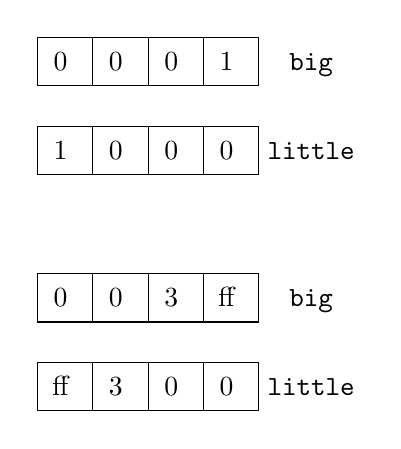
\begin{tikzpicture}[align=left, cell/.style={rectangle,draw=black},
            space/.style={minimum height=1.5em,matrix of nodes,row sep=-\pgflinewidth,column sep=-\pgflinewidth,column 1/.style={font=\ttfamily}},text depth=0.5ex,text height=2ex,nodes in empty cells]

            \matrix (endian)[space, row sep=0.5cm, column 5/.style={font=\ttfamily},column 2/.style={nodes={cell,minimum width=2em}},column 3/.style={nodes={cell,minimum width=2em}},column 4/.style={nodes={cell,minimum width=2em}},column 1/.style={nodes={cell,minimum width=2em}}]
            {
               0 & 0 & 0 & 1 & big\\
               1 & 0 & 0 & 0 & little\\
            };
            \matrix [space, row sep=0.5cm, column 5/.style={font=\ttfamily},column 2/.style={nodes={cell,minimum width=2em}},column 3/.style={nodes={cell,minimum width=2em}},column 4/.style={nodes={cell,minimum width=2em}},column 1/.style={nodes={cell,minimum width=2em}}, below=1cm of endian] 
            {
               0 & 0 & 3 & ff & big\\
               ff & 3 & 0 & 0 & little\\
            };
         \end{tikzpicture}
      \end{column}
   \end{columns}
\end{frame}
\note[itemize] {
\item El byte m\'as significativo se lee/escribe primero (o esta primero en la memoria) en las arquitecturas big endian.
\item Por el contrario en las arquitecturas little endian es el byte menos significativo quien esta primero en la memoria.
\item El endianess es irrelevante si siempre trabajamos los \lstinline[style=normal]!int!s como n\'umeros pero se vuelve relevante en el momento que queremos interpretar un \lstinline[style=normal]!int! como una tira de bytes (\lstinline[style=normal]!char*!) o viceversa. Y esto es necesario cuando queremos escribir un n\'umero en un archivo binario o enviarlo por la red a otra m\'aquina a traves de un socket!
\item Siempre hay que especificar el endianess en que se guardan/envian los datos. 
\item Obviamente lo mencionado aqui para los \lstinline[style=normal]!int!s aplica para el resto de los objetos en memoria, como los \lstinline[style=normal]!short!s
}

\begin{frame}[fragile]{Endianess: representaci\'on en memoria}
Se puede cambiar el endianess de una variable \lstinline[style=normal]!short int! y \lstinline[style=normal]!int!
del endianess nativo o "del host" a big endian o "el endianess de la red" y viceversa:
       \begin{itemize}
           \item Host to Network
         \begin{lstlisting}[style=normal]
htons(short int) htonl(int)
        \end{lstlisting}
           \item Network to Host
         \begin{lstlisting}[style=normal]
ntohs(short int) ntohl(int)
        \end{lstlisting}
   \end{itemize}
\end{frame}
\note[itemize] {
\item Para hacer uso de esas funciones hay que hacer \lstinline[style=normal]!\#include <arpa/inet.h>!.
}

\subsection{Segmentos de Memoria}
% Stack Heap Data Code
\begin{frame}[fragile,label=SM]{Segmentos de memoria}
   \begin{itemize}
      \item<1-> Code segment: de solo lectura y ejecutable, a donde va el c\'odigo y las constantes.
      \item<2-> Data segment: variables creadas al inicio del programa y son v\'alidas hasta que este termina; pueden ser de acceso global o local.
      \item<3-> Stack: variables creadas al inicio de una llamada a una funci\'on y destruidas autom\'aticamente cuando esta llamada termina.
      \item<4-> Heap: variables cuya duraci\'on esta controlada por el programador (run-time).
   \end{itemize}
\end{frame}
\begin{frame}[fragile,label=LS]{Duraci\'on y visibilidad (lifetime and scope)}
   \begin{itemize}
       \item<1-> Duraci\'on (lifetime): tiempo desde que a la variable se le reserva memoria hasta que esta es liberada. Determinado por el segmento de memoria que se usa.
       \item<2-> Visibilidad (scope): Cuando una variable se la puede acceder y cuando esta oculta.
   \end{itemize}
\end{frame}
% static (variables locales/globales y funciones)
\begin{frame}[fragile]{Asignaci\'on del lifetime y scope}
         \begin{lstlisting}[style=dimmided]
@int g = 1;@@
static int l = 1;@@
extern char e;@
@
void Fa() { }@@
static void Fb() { }@@
void Fc();@

void foo(@int arg@) {@
   int a = 1;@@
   static int b = 1;@
   @
   void * p = malloc(4);
   free(p);@
   @
   char *c = "ABC";@@
   char ar[] = "ABC";@
}
         \end{lstlisting}
\end{frame}
\begin{frame}[fragile]{Asignaci\'on del lifetime y scope}
         \begin{lstlisting}[style=normal]
int g = 1;          // Data segment; scope global
static int l = 1;   // Data segment; scope local (este file)
extern char e;      // No asigna memoria (es un nombre)

void Fa() { }        // Code segment; scope global
static void Fb() { } // Code segment; scope local (este file)
void Fc();           // No asigna memoria (es un nombre)

void foo(int arg) {  // Argumentos y retornos son del stack
   int a = 1;        // Stack segment; scope local (func foo)
   static int b = 1; // Data segment; scope local (func foo)

   void * p = malloc(4); // p en el Stack; apunta al Heap
   free(p);              // liberar el bloque explicitamente!!

   char *c = "ABC";   // c en el Stack; apunta al Code Segment
   char ar[] = "ABC"; // es un array con su todo en el Stack
} // fin del scope de foo: las variables locales son liberadas
         \end{lstlisting}
\end{frame}
\begin{frame}[fragile]{El donde importa!}
         \begin{lstlisting}[style=normal]

void f() {
   char *a = "ABC";
   char b[] = "ABC";

   b[0] = 'X';
   a[0] = 'X';  // segmentation fault
}
         \end{lstlisting}
\end{frame}
\note[itemize] {
\item Como el puntero "a" apunta al Code Segment y este es de solo lectura, tratar de modificarlo termina en un Segmentation Fault
}

\section{Punteros}
\subsection{Punteros}
% simples
\begin{frame}[fragile]{Punteros}
         \begin{lstlisting}[style=normal]
int *p;    // p es un puntero a int
           // (p guarda la direccion de un int)

int i = 1;
p = &i;    // &i es la direccion de la variable i

*p = 2;    // *p dereferencia o accede a la memoria
           // cuya direccion esta guardada en p

/* i == 2 */

         \end{lstlisting}
         \begin{lstlisting}[style=normal]

char buf[512];
write(&buf[0], 512);

         \end{lstlisting}
\end{frame}

% aritmetica de punteros
\begin{frame}[fragile]{Aritm\'etica de punteros}
         \begin{lstlisting}[style=normal]
int a[10];
int *p;

p = &a[0];

*p       // a[0]
*(p+1)   // a[1]


int *p;
p+1      // movete sizeof(int) bytes (4)

char *c;
c+2      // movete 2*sizeof(char) bytes (2)

         \end{lstlisting}
\end{frame}
\note[itemize] {
\item La notaci\'on de array (indexado) y la aritm\'etica de punteros son escencialmente lo mismo.
\item La aritm\'etica de punteros se basa en el tama\~no de los objetos a los que se apunta al igual que el indexado de un array.
}

% punteros a funcion
\begin{frame}[fragile]{Punteros a funciones (al code segment)}
         \begin{lstlisting}[style=normal]
int g(char) {}

int (*p)(char);
p = &g;
         \end{lstlisting}
\pause
         \begin{lstlisting}[style=normal]
#include <stdlib.h>
void qsort(void *base,
           size_t nmemb,
           size_t size,

           int (*cmp)(const void *, const void *)
          );

int cmp_personas(const void* a, const void* b) {
    struct Persona *pa = (struct Persona*)a;
    struct Persona *pb = (struct Persona*)b;

    return pa->edad - pb->edad;
}

         \end{lstlisting}
\end{frame}


\subsection{Typedef}
% como leer la bizarra notacion de punteros de C/C++
\begin{frame}[fragile]{Como leer la bizarra notaci\'on de punteros en C/C++}
         \begin{lstlisting}[style=dimmided]
@/* Ejemplo 1 */
char *a[10];@@
      a        // "a"
     *a        // "a" apunta a
char *a        // "a" apunta a char
char *a[10];   // "a" apunta a char (10 de esos)

char *a[10];   // "a" es un array de 10 de esos, o sea
               // "a" es un array de 10 punteros a char
@
         \end{lstlisting}
\end{frame}
\begin{frame}[fragile]{Como leer la bizarra notaci\'on de punteros en C/C++}
         \begin{lstlisting}[style=dimmided]
@/* Ejemplo 2 */
char (*c)[10];@@
       c       // "c"
      *c       // "c" apunta a
     (*c) == X // llamemos "X" a (*c) temporalmente
@@
char X[10];
char X[10];    // "X" es un char (10 de esos)

char X[10];    // "X" es un array de 10 char
@@char (*c)[10]; // "c" apunta a un array de 10 char
@
         \end{lstlisting}
\end{frame}
\begin{frame}[fragile]{Como leer la bizarra notaci\'on de punteros en C/C++}
         \begin{lstlisting}[style=dimmided]
@/* Ejemplo 3: modo dios */
char (*f)(int)[10];@@
       f            // "f"
      *f            // "f" apunta a
     (*f) == X
@@
char X(int)[10];@@
char X(int)         // es la firma de una funcion,
                    // asi que vuelvo un paso para atras
char (*f)(int)      // entonces esto es un puntero a funcion
                    // cuya firma recibe un int y retorna
                    // un char
@@
char (*f)(int)[10]; // puntero a funcion, 10 de esos
char (*f)(int)[10]; // f es un array de 10 punteros a funcion,
                    // que reciben un int y retornan un chars
@
         \end{lstlisting}
\end{frame}

% typedef
\begin{frame}[fragile]{Simplificando la notaci\'on}{}
         \begin{lstlisting}[style=normal]
        char *X[10];   // la variable "X" es un array de
                       // 10 punteros a char

         \end{lstlisting}
         \begin{lstlisting}[style=normal]
typedef char *X[10];   // el tipo "X" es un array de
                       // 10 punteros a char

X my_array;            // es una alias, decir "X" es como decir
char *my_array[10];    // "array de 10 punteros a char"

         \end{lstlisting}
\end{frame}
\begin{frame}[fragile]{Simplificando la notaci\'on}{}
Si quiero una variable que sea un array de punteros a funci\'on que no reciban ni retornen nada?
         \begin{lstlisting}[style=normal]
        void (*X)();   // la variable "X" es un puntero a
                       // funcion

         \end{lstlisting}
         \begin{lstlisting}[style=normal]
typedef void (*X)();   // el tipo "X" es un puntero a
                       // funcion

X f[10];               // f es una array de 10 X, entonces
                       // f es una array de 10 punteros
                       // a funcion
         \end{lstlisting}
\end{frame}

\section{Buffer overflows}
\subsection*{}
\begin{frame}[fragile]{Smash the stack for fun and profit}
         \begin{lstlisting}[style=normal]
// compilar con el flag -fno-stack-protector
#include <stdio.h>

int main(int argc, char *argv[]) {
    int cookie = 0;
    char buf[10];

    printf("buf: %08x cookie: %08x\n", buf, &cookie);
    gets(buf);

    if (cookie == 0x41424344) {
        printf("You win!\n");
    }

    return 0;
} // Insecure Programming
         \end{lstlisting}
\end{frame}
\note[itemize] {
\item Es claro que al inicializar \lstinline[style=normal]!cookie! a cero nunca se va a imprimir \lstinline[style=normal]?"You win!"?... o si?
\item \lstinline[style=normal]!gets! lee de la entrada est\'andar hasta encontrar un \lstinline[style=normal]!'\\n'! y lo que leea lo escribira en el buffer \lstinline[style=normal]!buf!. Pero si el input es m\'as grande que el buffer, \lstinline[style=normal]!gets! escribira por fuera de este y sobreescribira todo el stack lo que se conoce como Buffer Overflow.
\item Para hacer que el programa entre al \lstinline[style=normal]!if! e imprima \lstinline[style=normal]?"You win!"? se debe forzar a un buffer overflow con un input crafteado:
\item Debe tener 10 bytes de m\'inima para ocupar el buffer \lstinline[style=normal]!buf!.
\item Posiblemente deba tener algunos bytes adicionales para ocupar el posible espacio de padding usado para alinear las variables.
\item Luego se debe escribir los 4 bytes que sobreescribiran \lstinline[style=normal]!cookie! pero cuidado, dependiendo de la arquitectura y flags del compilador \lstinline[style=normal]!sizeof(int)! puede no ser 4.
\item Suponiendo que sean 4 bytes, hay que escribir el n\'umero \lstinline[style=normal]!0x41424344! byte a byte y el orden dependera del endianess: \lstinline[style=normal]!"ABCD"! en big endian, \lstinline[style=normal]!"DCBA"! en little endian.
}

\begin{frame}[fragile]{Buffer overflow}{}
   \begin{itemize}
      \item Funciones inseguras que no ponen un l\'imite en el tama\~no del buffer que usan. No usarlas!
         \begin{lstlisting}[style=normal]
gets(buf);
strcpy(dst, src);
         \end{lstlisting}

     \item Reemplazarlas por funciones que s\'i permiten definir un l\'imite, pero es responsabilidad del programador poner un valor coherente! 
         \begin{lstlisting}[style=normal]
getline(buf, max_buf_size, stream);
strncpy(dst, src, max_dst_size);
         \end{lstlisting}
   \end{itemize}
\end{frame}
\begin{frame}[fragile]{Challenge: hacer que el programa imprima "You win!"}
         \begin{lstlisting}[style=normal]
// compilar con el flag -fno-stack-protector
#include <stdio.h>

int main(int argc, char *argv[]) {
    int cookie = 0;
    char buf[10];

    printf("buf: %08x cookie: %08x\n", buf, &cookie);
    gets(buf);

    if (cookie == 0x41424344) {
        printf("You loose!\n");
    }

    return 0;
} // Insecure Programming
         \end{lstlisting}
\end{frame}

\appendix
\section<presentation>*{\appendixname}
\subsection<presentation>*{Referencias}

\begin{frame}[allowframebreaks]
   \frametitle<presentation>{Referencias}

   \begin{thebibliography}{10}

         \beamertemplatebookbibitems
         % Start with overview books.

      \bibitem{Stroustrup}
         Bjarne Stroustrup.
         \newblock {\em The C++ Programming Language}.
         \newblock Addison Wesley, Fourth Edition.

         \beamertemplatearticlebibitems

      \bibitem{man page: gets strcpy htons qsort}
         man page: gets strcpy htons qsort

      \bibitem{Insecure Programming}
         Insecure Programming

         % Followed by interesting articles. Keep the list short.

   \end{thebibliography}
\end{frame}

\end{document}


